% Created 2025-10-20 seg 09:51
% Intended LaTeX compiler: pdflatex
\documentclass[12pt,xcolor=dvipsnames,presentation,aspectratio=169]{beamer}
\usepackage[utf8]{inputenc}
\usepackage[T1]{fontenc}
\usepackage{graphicx}
\usepackage{longtable}
\usepackage{wrapfig}
\usepackage{rotating}
\usepackage[normalem]{ulem}
\usepackage{amsmath}
\usepackage{amssymb}
\usepackage{capt-of}
\usepackage{hyperref}
\usedescriptionitemofwidthas{bl}
\usepackage{ifthen,figlatex,amsmath,amstext,xspace}
\usepackage{boxedminipage,xspace,multicol}
\usepackage{subfigure}
\usepackage{fancyvrb}
\usetheme{Madrid}
\usecolortheme[named=BrickRed]{structure}
%\usepackage[colorlinks=true,citecolor=pdfcitecolor,urlcolor=pdfurlcolor,linkcolor=pdflinkcolor,pdfborder={0 0 0}]{hyperref}
\usepackage[round-precision=3,round-mode=figures,scientific-notation=true]{siunitx}
\setbeamertemplate{footline}[frame number]
\setbeamertemplate{navigation symbols}{}
\usepackage{DejaVuSansMono}
%\AtBeginDocument{
%  \definecolor{pdfurlcolor}{rgb}{0,0,0.6}
%  \definecolor{pdfcitecolor}{rgb}{0,0.6,0}
%  \definecolor{pdflinkcolor}{rgb}{0.6,0,0}
%  \definecolor{light}{gray}{.85}
%  \definecolor{vlight}{gray}{.95}
%}
\usepackage{appendixnumberbeamer}
\usepackage{relsize}
\usepackage{color,colortbl}
\definecolor{gray98}{rgb}{0.98,0.98,0.98}
\definecolor{gray20}{rgb}{0.20,0.20,0.20}
\definecolor{gray25}{rgb}{0.25,0.25,0.25}
\definecolor{gray16}{rgb}{0.161,0.161,0.161}
\definecolor{gray60}{rgb}{0.6,0.6,0.6}
\definecolor{gray30}{rgb}{0.3,0.3,0.3}
\definecolor{bgray}{RGB}{248, 248, 248}
\definecolor{amgreen}{RGB}{77, 175, 74}
\definecolor{amblu}{RGB}{55, 126, 184}
\definecolor{amred}{RGB}{228,26,28}
\usepackage[procnames]{listings}
\lstset{ %
backgroundcolor=\color{gray98},    % choose the background color; you must add \usepackage{color} or \usepackage{xcolor}
basicstyle=\tt\prettysmall,      % the size of the fonts that are used for the code
breakatwhitespace=false,          % sets if automatic breaks should only happen at whitespace
breaklines=true,                  % sets automatic line breaking
showlines=true,                  % sets automatic line breaking
captionpos=b,                     % sets the caption-position to bottom
commentstyle=\color{gray30},      % comment style
extendedchars=true,               % lets you use non-ASCII characters; for 8-bits encodings only, does not work with UTF-8
frame=single,                     % adds a frame around the code
keepspaces=true,                  % keeps spaces in text, useful for keeping indentation of code (possibly needs columns=flexible)
keywordstyle=\color{amblu},       % keyword style
procnamestyle=\color{amred},       % procedures style
language=C,             % the language of the code
numbers=none,                     % where to put the line-numbers; possible values are (none, left, right)
numbersep=5pt,                    % how far the line-numbers are from the code
numberstyle=\tiny\color{gray20}, % the style that is used for the line-numbers
rulecolor=\color{gray20},          % if not set, the frame-color may be changed on line-breaks within not-black text (e.g. comments (green here))
showspaces=false,                 % show spaces everywhere adding particular underscores; it overrides 'showstringspaces'
showstringspaces=false,           % underline spaces within strings only
showtabs=false,                   % show tabs within strings adding particular underscores
stepnumber=2,                     % the step between two line-numbers. If it's 1, each line will be numbered
stringstyle=\color{amdove},       % string literal style
tabsize=2,                        % sets default tabsize to 2 spaces
% title=\lstname,                    % show the filename of files included with \lstinputlisting; also try caption instead of title
procnamekeys={call}
}
\newcommand{\prettysmall}{\fontsize{6}{8}\selectfont}
\newcommand{\quitesmall}{\fontsize{8}{10}\selectfont}
\usepackage{tikzsymbols}
\def\smiley{\Smiley[1][green!80!white]}
\def\frowny{\Sadey[1][red!80!white]}
\def\winkey{\Winkey[1][yellow]}
\def\smileyitem{\setbeamertemplate{itemize item}{\scriptsize\raise1.25pt\hbox{\donotcoloroutermaths\color{black}$\smiley$}}}
\def\frownyitem{\setbeamertemplate{itemize item}{\scriptsize\raise1.25pt\hbox{\donotcoloroutermaths\color{black}$\frowny$}}}
\def\restoreitem{\setbeamertemplate{itemize item}[ball]}
\def\smileysubitem{\setbeamertemplate{itemize subitem}{\scriptsize\raise1.25pt\hbox{\donotcoloroutermaths\color{black}$\smiley$}}}
\def\frownysubitem{\setbeamertemplate{itemize subitem}{\scriptsize\raise1.25pt\hbox{\donotcoloroutermaths\color{black}$\frowny$}}}
\def\restoresubitem{\setbeamertemplate{itemize subitem}[ball]}
\setbeamerfont{title}{size=\normalsize}
\usetheme{Madrid}
\usecolortheme{default}
\usefonttheme{professionalfonts}
\author{Otho José Sirtoli Marcondes, Philippe O. A. Navaux, Lucas Mello Schnorr}
\date{Ocotber 2025}
\title{Impact of Data Distribution and Schedulers for the LU Factorization on Multi-Core Clusters Impact of Data Distribution and Schedulers for the LU Factorization on Multi-Core Clusters}
\hypersetup{
 pdfauthor={Otho José Sirtoli Marcondes, Philippe O. A. Navaux, Lucas Mello Schnorr},
 pdftitle={Impact of Data Distribution and Schedulers for the LU Factorization on Multi-Core Clusters Impact of Data Distribution and Schedulers for the LU Factorization on Multi-Core Clusters},
 pdfkeywords={},
 pdfsubject={},
 pdfcreator={Emacs 28.1 (Org mode 9.7.26)}, 
 pdflang={English}}
\begin{document}

\urlstyle{sf}
\let\alert=\structure
\let\epsilon=\varepsilon
\let\leq=\leqslant
\let\geq=\geqslant

{%\setbeamertemplate{footline}{} 

\author{Otho José Sirtoli Marcondes, Lucas Mello Schnorr, Phillipe Olivier Alexandre Navaux \newline Instituto de Informática, UFRGS}

\date{Ocotber 28th, 2025 \\\smallskip}

\titlegraphic{\vspace{-.2cm
    
\includegraphics[scale=0.12]{./logo/ppgc.png}\hspace{2cm}
    
\includegraphics[scale=1.6]{./logo/ufrgs.png}}}

\maketitle
\section{Introduction and Motivation}
\label{sec:org4ed9cdb}
\begin{frame}[label={sec:org6ffc0f5}]{Context}
\begin{itemize}
\item HPC is the backbone for groundbreaking research and innovation across numerous scientific and engineering disciplines.
\item Modern clusters have thousands of multi-core nodes.
\item Dense linear algebra (e.g., LU factorization) is a core workload.
\end{itemize}
\end{frame}
\begin{frame}[label={sec:orgc701df0}]{Introduction and Motivation}
Load balancing across nodes is a critical challenge.
\begin{itemize}
\item Static data distribution: excellent data locality but lacks adaptability.
\item Dynamic scheduling: great adaptability but incurs overhead.
\item Hybrid strategies aim to combine both efficiently (StarPU-MPI and CHAMELEON).
\end{itemize}
Objective
\begin{itemize}
\item Analyze how \alert{data distribution} and \alert{scheduling heuristics} affect LU factorization performance.
\end{itemize}
\end{frame}
\section{Related Work}
\label{sec:orgd8a20ba}
\begin{frame}[label={sec:org6bdcb9f}]{Static Data Distribution}
\begin{itemize}
\item \alert{Block-Cyclic (BC)} used in ScaLAPACK, HPL benchmark.
\item Balances computation and communication via P×Q grid.
\item Limitations with prime node counts or heterogeneous resources.
\end{itemize}
\begin{center}
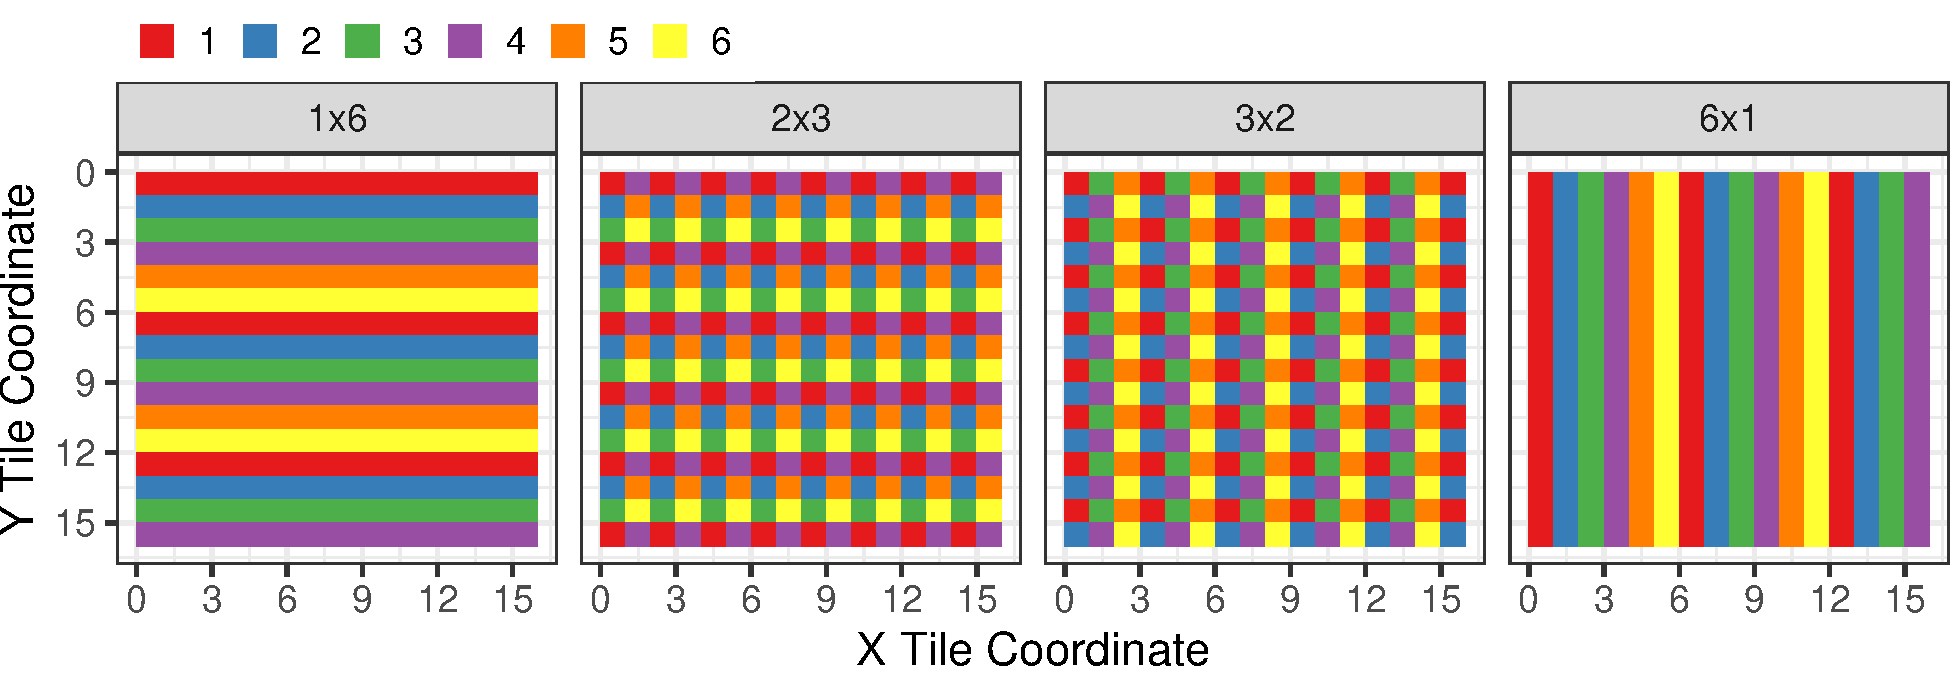
\includegraphics[height=2.5cm]{../img/bc.pdf}
\end{center}
\end{frame}
\begin{frame}[label={sec:org3f0c482}]{Task-Based Runtime Systems}
\begin{itemize}
\item Frameworks: StarPU, PaRSEC, OmpSs.
\item Express computations as task DAGs.
\item Adaptability and performance portability.
\item Schedulers dynamically assign tasks.
\end{itemize}
\end{frame}
\section{Experimental Setup}
\label{sec:org05cc1aa}
\begin{frame}[label={sec:org5261af6}]{Hardware Environment}
\begin{center}
\begin{tabular}{ll}
Resource & Specification\\
\hline
Cluster & PCAD @ INF/UFRGS\\
Nodes & 6\\
Cores per node & 24 (2×12 Xeon Silver 4116)\\
Memory per node & 96 GB DDR4\\
Network & 10G Ethernet (X540-AT2)\\
\end{tabular}
\end{center}
\end{frame}
\begin{frame}[label={sec:org23ee8e2}]{Software Environment}
\begin{itemize}
\item CHAMELEON 1.3.0 for dense linear algebra.
\item StarPU-MPI 1.4.7 runtime system.
\item OpenMPI 4 transport layer.
\item GNU Guix for reproducible package management.
\item Data analysis in R suing StarVZ framework.
\end{itemize}
\end{frame}
\section{Methods}
\label{sec:orgc1fc23b}
\begin{frame}[label={sec:org9e38ac0}]{Application: LU Factorization}
\begin{itemize}
\item Decomposes matrix A into L (lower) and U (upper).
\item Kernels used:
\begin{itemize}
\item DGEMM – matrix multiplication
\item DTRSM – triangular solve
\item DGETRF\_NOPIV – LU without pivoting
\end{itemize}
\item Hybrid execution:
\begin{itemize}
\item Static inter-node block distribution
\item Dynamic intra-node scheduling via StarPU
\end{itemize}
\end{itemize}
\end{frame}
\begin{frame}[label={sec:org16bcab8},fragile]{Experimental Design}
 Square matrix size of 14.4K (double precision).
\begin{enumerate}
\item \alert{Phase 1}: Tile size tuning (128–1600)
\item \alert{Phase 2}: Full factorial 4×4 experiment
\begin{itemize}
\item Schedulers: lws, random, dmda, dmdas
\item Distributions: 1×6, 2×3, 3×2, 6×1
\end{itemize}
\item \alert{Phase 3}: Detailed trace analysis with StarVZ
\begin{itemize}
\item Fixed \texttt{lws} scheduler
\item Varying PxQ (BC) parameters.
\end{itemize}
\end{enumerate}
\end{frame}
\section{Results — Optimal Block Size}
\label{sec:org19ab87a}
\begin{frame}[label={sec:org652d67c},fragile]{Preliminary Study}
 \begin{itemize}
\item Tested 10 tile sizes with \texttt{lws} scheduler.
\item Best performance at \alert{360×360} blocks.
\end{itemize}

\begin{center}
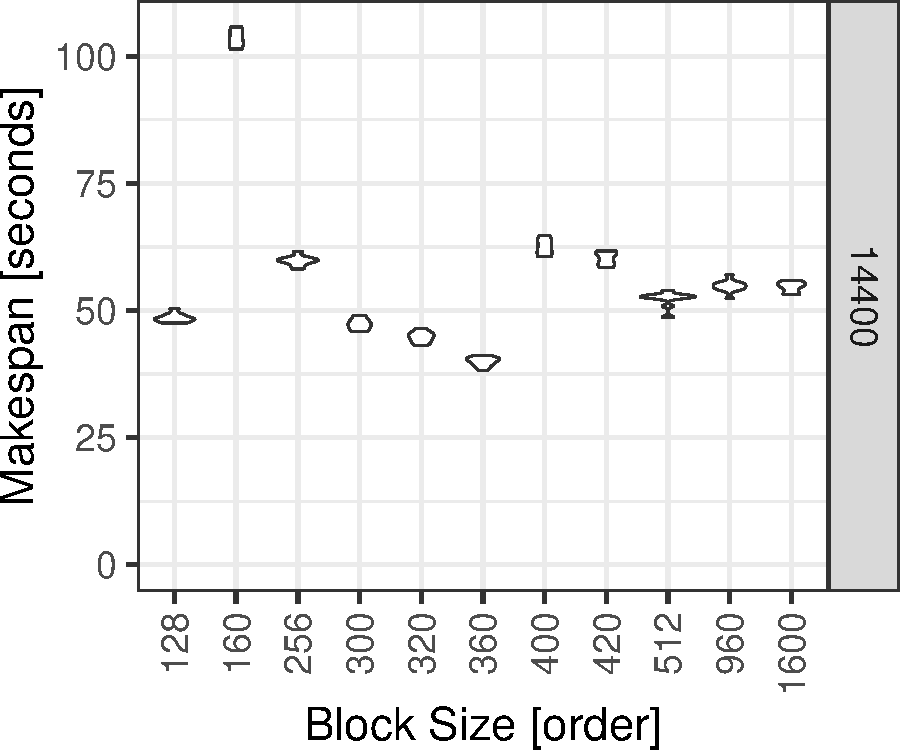
\includegraphics[width=0.3\textwidth]{../img/block-size.pdf}
\end{center}
\end{frame}
\section{Results — Scheduler and Data Partition}
\label{sec:org8ce85b1}
\begin{frame}[label={sec:orgfd076bb}]{Overview of the Comparison}
\begin{itemize}
\item Varying data distribution and schedulers.
\item 1\texttimes{}6 and 6\texttimes{}1: \(\approx\)3900 MPI operations.
\item 2\texttimes{}3 and 3\texttimes{}2: \(\approx\)2300 MPI operations.
\item Similar makespans across different data distributions and schedulers.
\end{itemize}

\begin{center}
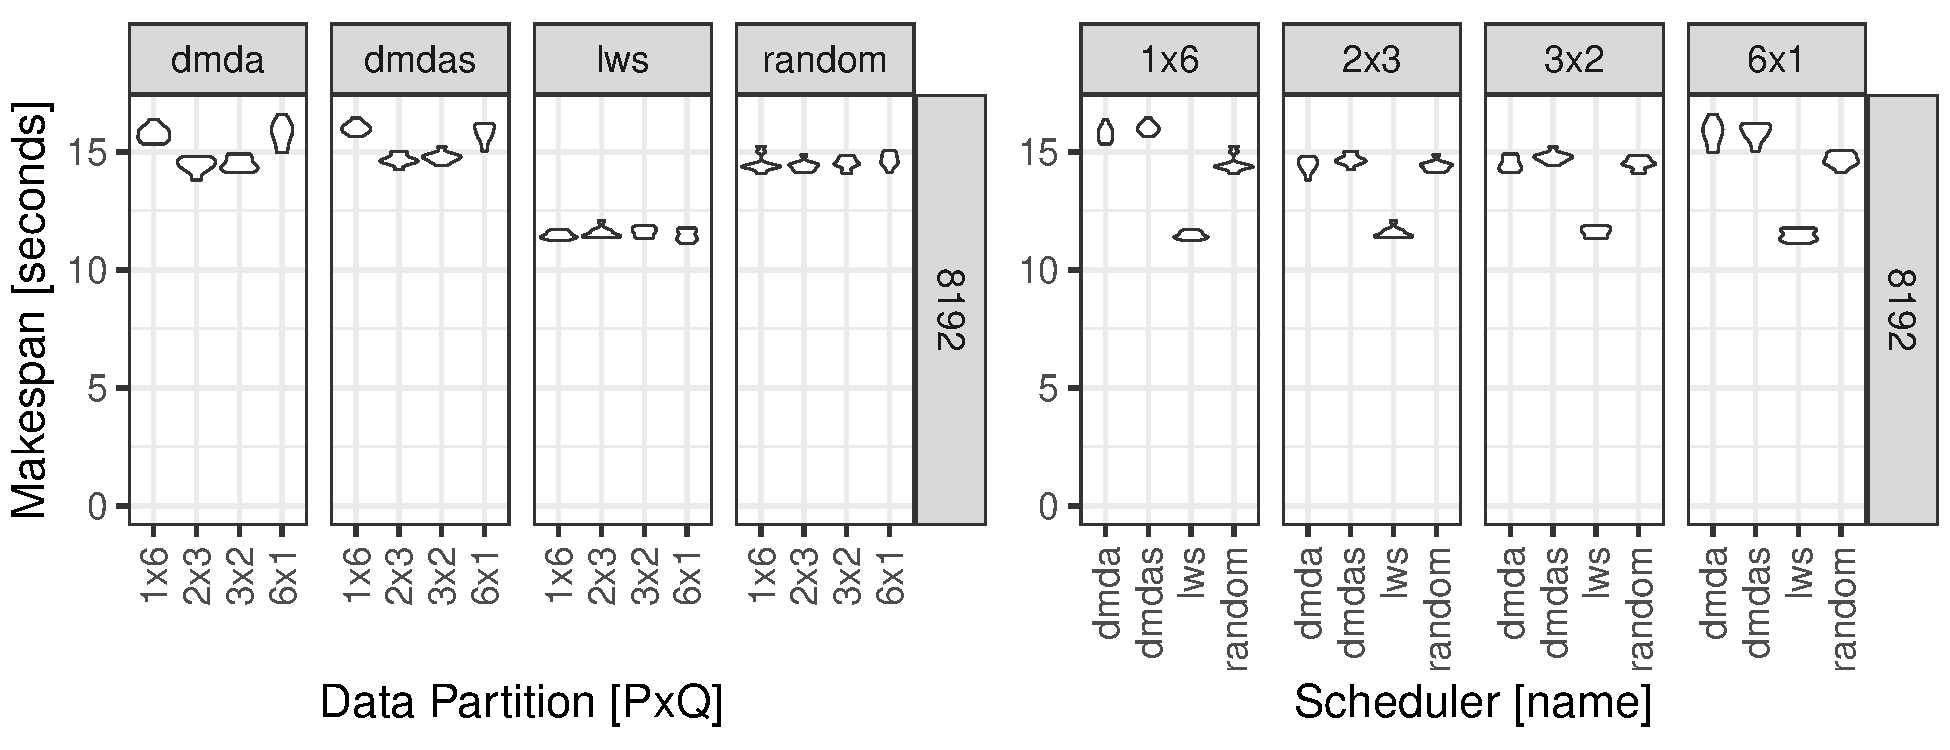
\includegraphics[width=0.3\textwidth]{../img/distrib-scheduler.pdf}
\end{center}
\end{frame}
\section{Results — OpenMPI Delays}
\label{sec:org31a2bd7}
\begin{frame}[label={sec:org0452a6e},fragile]{OpenMPI Delays}
 \begin{itemize}
\item Fixed \texttt{lws} scheduler, varying data distributions.
\item More dense behavior of \texttt{dgemm} tasks until 10s.
\begin{itemize}
\item 1×6 (worst): mean idle \(\approx\)1500 ms
\item 2×3 (best): mean idle \apporx800 ms
\end{itemize}
\item Bottleneck from network latency, not algorithmic imbalance.
\end{itemize}
\end{frame}
\begin{frame}[label={sec:orgc23ae19}]{OpenMPI Delays}
\begin{center}
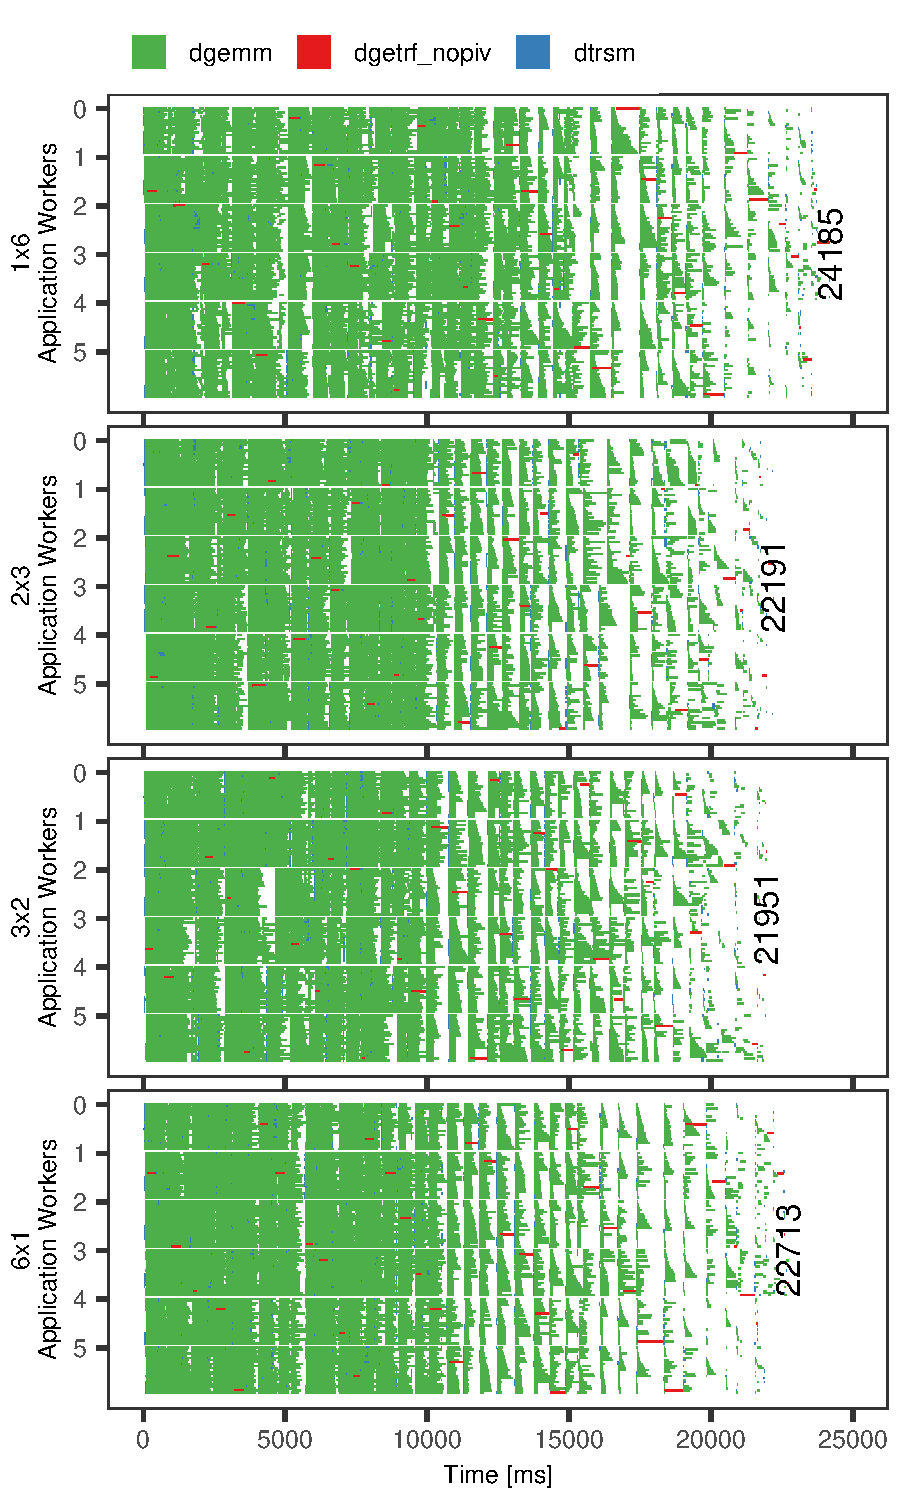
\includegraphics[width=0.3\textwidth]{../img/lws-all_pq-traces.pdf}
\end{center}
\end{frame}
\section{Results — Scheduler Comparison}
\label{sec:org159c3df}
\begin{frame}[label={sec:orgaa7835d},fragile]{Schedulers Comparison}
 \begin{itemize}
\item Fixed 3×2 distribution, \texttt{lws} and \texttt{dmdas} schedulers.
\item Per-node optimistic makespan (ABE):
\begin{itemize}
\item \(\approx\)14605 ms for \texttt{lws}
\item \(\approx\)15045 ms for \texttt{dmdas}
\end{itemize}
\item LWS temporal gaps between tasks \(\approx\)7841 ms; \texttt{dmdas} \(\approx\)9154 ms.
\item 200 more outlier tasks in \texttt{dmdas} explain longer runtime.
\end{itemize}

\begin{center}
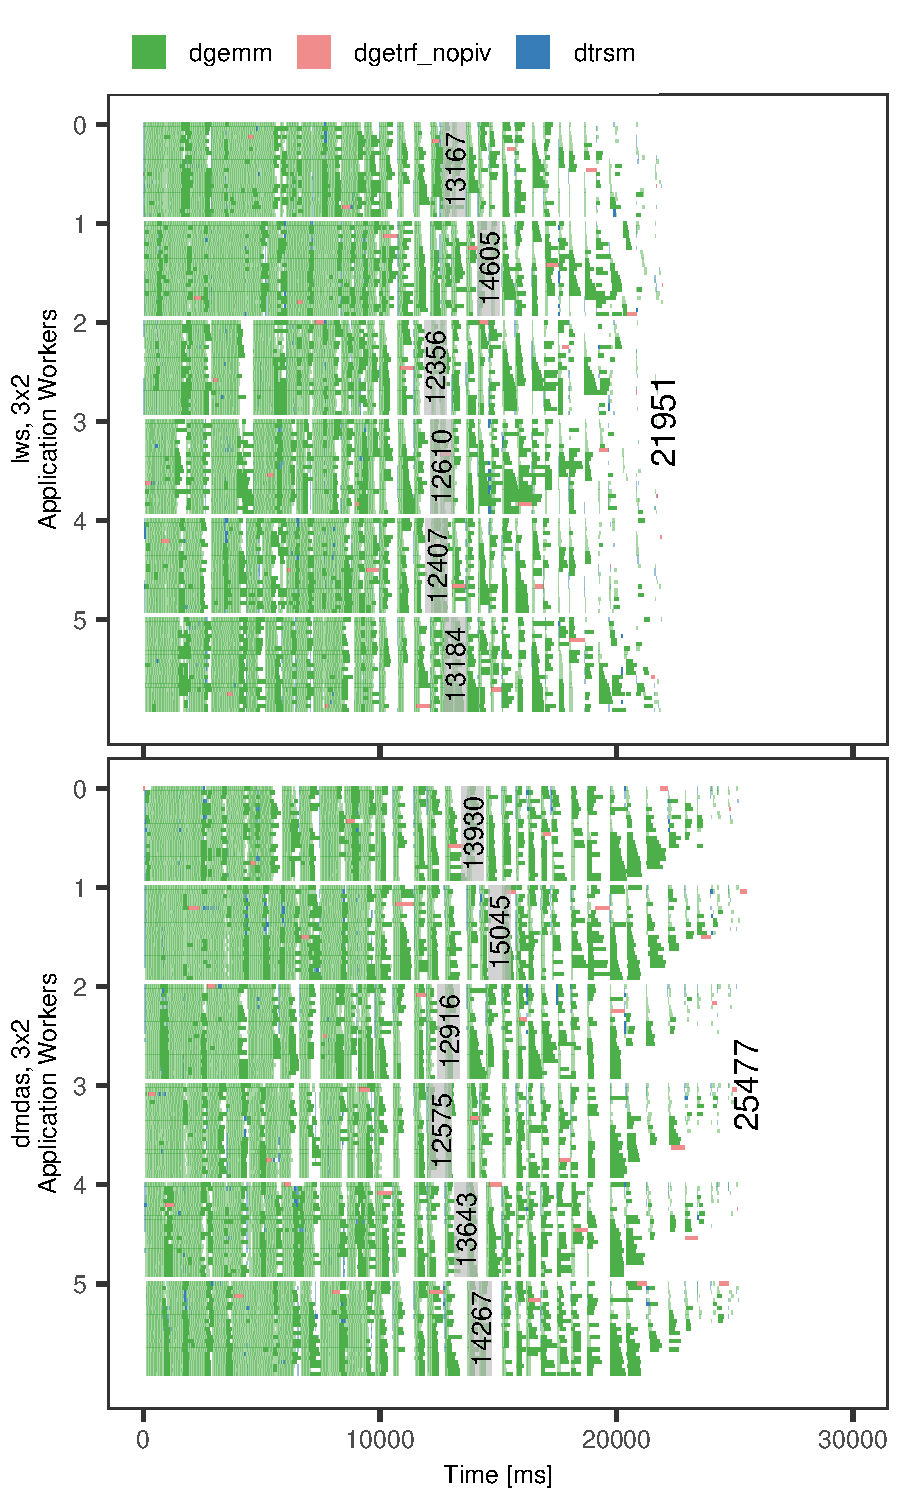
\includegraphics[width=0.4\textwidth]{../img/lws-vs-dmdas-3x2-openmpi-traces.pdf}
\end{center}
\end{frame}
\section{Results — Data Distribution Similarities}
\label{sec:org2bfa49e}
\begin{frame}[label={sec:orgaa06962}]{Data distribution similarities}
\begin{itemize}
\item Makespan difference <3\%.
\item ABE difference between nodes 1 and 2:
\begin{itemize}
\item 3\texttimes{}2: \(\approx\)2249 ms
\item 6\texttimes{}1: \(\approx\)2194 ms
\end{itemize}
\item Similar load imbalance between the two.
\end{itemize}

\begin{center}
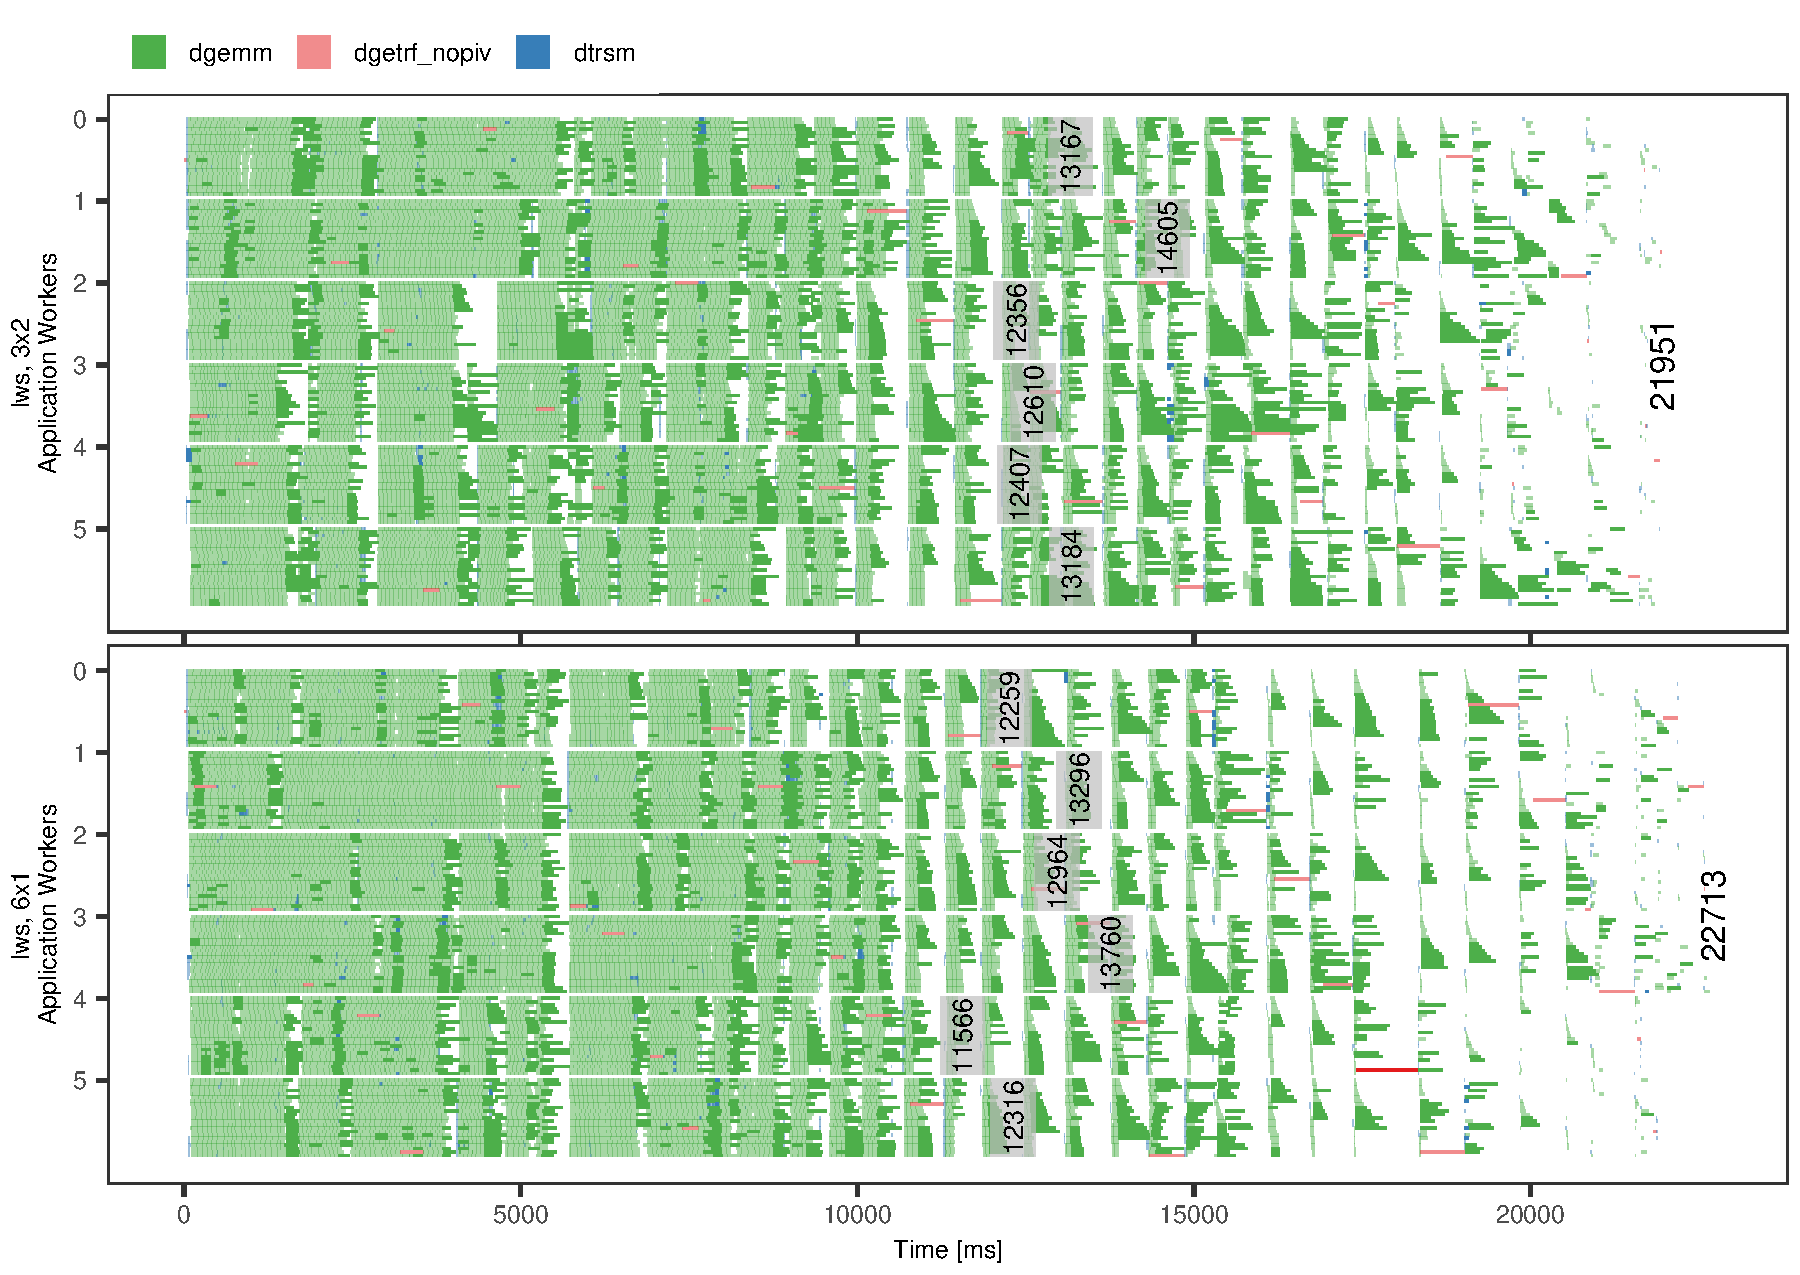
\includegraphics[width=0.45\textwidth]{../img/lws-3x2-versus-6x1-openmpi-traces.pdf}
\end{center}
\end{frame}
\section{Conclusion}
\label{sec:org4bb43ea}
\begin{frame}[label={sec:org1e5ebc1},fragile]{Conclusion and Future Work}
 \begin{itemize}
\item Impact of data distribution and scheduler heuristics.
\item \texttt{dmda} and \texttt{dmdas} presented similar performances.
\item \texttt{lws} best performing scheduler.
\item Data partition (P\timesQ) had minimal impact on performance.
\item Scale experiments using SimGrid simulation.
\item Study repetitive network delays in StarPU-MPI.
\end{itemize}
\end{frame}
\section{Acknowledgements}
\label{sec:org9df33f0}
\begin{frame}[label={sec:org3362039}]{Acknowledgments}
The experiments in this work used the PCAD infrastructure,
\url{http://gppd-hpc.inf.ufrgs.br}, at INF/UFRGS.  We also acknowledge the
Brazilian National Council for Scientific Technological Development
(CNPq) for their financial scholarship support. This study was
financed in part by the Coordenação de Aperfeiçoamento de Pessoal de
Nível Superior - Brasil (CAPES) - Finance Code 001, the FAPERGS
(16/354-8, 16/348-8), Petrobras (2020/00182-5).
\end{frame}
\section{Contact}
\label{sec:orgbb5f385}
\begin{frame}[label={sec:orge62ab3e}]{Contact}
\begin{center}
Thank you for your attention!
\end{center}

\begin{center}
Otho José Sirtoli Marcondes <otho.marcondes@inf.ufrgs.br>

Lucas Mello Schnorr <schnorr@inf.ufrgs.br>

Phillipe Olivier Alexandre Navaux <navaux@inf.ufrgs.br>
\end{center}
\end{frame}
\end{document}
